\chapter{Controle Bancário: Versão 3}\label{autorizacao}

Neste  capítulo,   dando  continuidade   ao  desenvolvimento  em   Grails,  será
apresentado o processo  de desenvolvimento da terceira versão  da aplicação {\bf
  ControleBancario}. Nessa versão são incorporadas as seguintes funcionalidades:

\begin{itemize}

\vspace{0.5cm}

\item Sintonia fina no controle de acesso:

\vspace{0.5cm}

\begin{itemize}

\vspace{0.5cm}

\item Atribuição de  papéis na criação das instâncias da  classe de domínio {\bf
  Gerente} e das instâncias das subclasses da classe {\bf Cliente}; 

\vspace{0.5cm}

\item Na segunda versão da  aplicação {\bf ControleBancario}, um cliente (físico
  ou jurídico)  pode acessar todas as  transações feitas em  contas (corrente ou
  poupança).  Na versão, discutida  nesse capítulo, clientes apenas terão acesso
  às transações realizadas nas contas (corrente ou poupança) a eles associadas;

\vspace{0.5cm}

\item  Se um  cliente possui  mais  de uma  conta (corrente  ou poupança),  será
  solicitado  que ele  escolha a  conta (corrente  ou poupança)  que  ele deseja
  acessar; 

\vspace{0.5cm}

\item Analogamente,  na segunda versão  da aplicação {\bf  ControleBancario}, um
  gerente  pode  acessar qualquer  conta  (corrente  ou  poupança).  Na  versão,
  discutida nesse capítulo, gerentes  apenas terão acesso às contas pertencentes
  à agência em que ele trabalha.

\end{itemize}

\vspace{0.5cm}

\item     Alteração     do    controlador     {\bf     Main},    definido     no
  Capítulo~\ref{autorizacao}, para refletir as mudanças relacionadas ao controle 
  de acesso;

\vspace{0.5cm}

\item  Alteração da  biblioteca  de marcas  {\it  LoginTagLibrary}, definida  no
  Capítulo~\ref{autorizacao}, para refletir as mudanças relacionadas ao controle
  de acesso; 

\vspace{0.5cm}

\item Acesso a um serviço {\it web}  que, dado um CEP como parâmetro, retorna as
  demais  informações de um  endereço (logradouro,  bairro, cidade,  etc). Essas
  informações  serão utilizadas  no  preenchimento automático  dos atributos  da
  classe de domínio {\bf Endereco}. 

\end{itemize}

\section{Configuração da aplicação} 

\vspace{0.5cm}

\noindent{\bf   Instalação   de    {\it   plugins}.}    Na   implementação   das
funcionalidades da aplicação  {\bf ControleBancario}, discutidas nesse capítulo,
será utilizado um  {\it plugin} Grails que adiciona  funcionalidades de clientes
REST. Ou seja,  ao utilizarmos esse {\it plugin}  será possível acessar serviços
web REST.\index{Plugins!rest} 

\vspace{0.2cm}

Conforme mencionado, desde  a versão 3 do Grails, a  inserção de dependências de
{\it  plugins} é  realizada no  arquivo  {\bf build.gradle}.   O conteúdo  desse
arquivo,  relacionado  à  configuração  de  dependências  de  {\it  plugins},  é
apresentado no Código~\ref{codBuildGradle3}.  

\vspace{0.2cm}

Dessa forma, para instalar  o plugin {\bf grails-datastore-rest-client} adicione
o comando \texttt{ compile "org.grails:grails-datastore-rest-client:5.0.0.RC2"},
descrevendo a  dependência, no arquivo {\bf  build.graddle} conforme apresentado
na linha 15 do Código~\ref{codBuildGradle3}. 

\begin{lstlisting}[numbers=left,  caption={\bf  build.gradle}, frame=trBL,
    float=htbp, label=codBuildGradle3, basicstyle =\footnotesize]
repositories {
    mavenLocal()
    maven { url "https://repo.grails.org/grails/core" }
}

dependencyManagement {
    imports {
        mavenBom "org.grails:grails-bom:$grailsVersion"
    }
    applyMavenExclusions false
}

dependencies {
    compile "org.springframework.boot:spring-boot-starter-logging"
    compile "org.springframework.boot:spring-boot-autoconfigure"
    compile "org.grails:grails-core"
    compile "org.springframework.boot:spring-boot-starter-actuator"
    compile "org.springframework.boot:spring-boot-starter-tomcat"
    compile "org.grails:grails-dependencies"
    compile "org.grails:grails-web-boot"
    compile "org.grails.plugins:cache"
    compile "org.grails.plugins:scaffolding"
    compile "org.grails.plugins:hibernate4"
    compile "org.hibernate:hibernate-ehcache"
    compile "org.grails.plugins:br-validation:0.3"
    compile "org.grails.plugins:spring-security-core:3.0.4"
    compile "org.grails:grails-datastore-rest-client:5.0.0.RC2"
    compile "org.grails.plugins:ajax-tags:1.0.0"
    console "org.grails:grails-console"
    profile "org.grails.profiles:web:3.1.4"
    runtime "org.grails.plugins:asset-pipeline"
    runtime "com.h2database:h2"
    runtime "org.postgresql:postgresql:9.3-1101-jdbc41"
    testCompile "org.grails:grails-plugin-testing"
    testCompile "org.grails.plugins:geb"
    testRuntime "org.seleniumhq.selenium:selenium-htmlunit-driver:2.47.1"
    testRuntime "net.sourceforge.htmlunit:htmlunit:2.18"
}
\end{lstlisting}

\section{Atribuição de papéis}

\vspace{0.5cm}

Na   segunda  versão   da   aplicação  {\bf   ControleBancario},  discutida   no
Capítulo~\ref{autenticacao}, os papéis são  atribuídos durante o {\it Bootstrap}
da aplicação  (Código~\ref{codBootStrap23}). Nessa terceira  versão da aplicação
{\bf ControleBancario}, a atribuição de papéis seguirá a abordagem discutida nas
próximas seções. 

\subsection{Classe de domínio Gerente X Papel {\bf ROLE\_GERENTE}}

\vspace{0.5cm}

Na  terceira   versão  da  aplicação   {\bf  ControleBancario},  o   papel  {\bf
  ROLE\_GERENTE} será atribuído automaticamente às todas instâncias da classe de
domínio {\bf Gerente}.  

\vspace{0.2cm}

Código~\ref{codSaveGerente}  mostra a  reimplementação da  ação {\bf  save()} do
controlador {\bf GerenteController} com o objetivo de atribuir automaticamente o 
papel  {\bf ROLE\_GERENTE}  a  todas as  instâncias  da classe  de domínio  {\bf
  Gerente}. Conforme  pode-se observar,  logo após a  operação de {\bf  save} na
instância  da classe  de  domínio  {\bf Gerente}  (linha~29),  essa instância  é
associada ao papel {\bf ROLE\_GERENTE} (linhas~31-33). 

\begin{lstlisting}[numbers=left,  caption=Controlador {\bf  Gerente}  (ação {\bf
      save()}), frame=trBL, float=htbp, label=codSaveGerente] 
package br.ufscar.dc.dsw

import static org.springframework.http.HttpStatus.*
import grails.transaction.Transactional
import org.springframework.security.access.annotation.Secured

@Secured('ROLE_ADMIN')
@Transactional(readOnly = true)
class GerenteController {

    static allowedMethods = [save: "POST", update: "PUT", delete: "DELETE"]

    // Demais a^çõ^es/m^é^todos do controlador GerenteController

    @Transactional
    def save(Gerente gerente) {
        if (gerente == null) {
            transactionStatus.setRollbackOnly()
            notFound()
            return
        }

        if (gerente.hasErrors()) {
            transactionStatus.setRollbackOnly()
            respond gerente.errors, view:'create'
            return
        }

        gerente.save flush:true

        def gerentePapel = Papel.findByAuthority("ROLE_GERENTE")
        
        UsuarioPapel.create(gerente, gerentePapel)
        
        request.withFormat {
            form {
                flash.message = message(code: 'default.created.message', 
                                        args: [message(code: 'gerente.label', 
                                        default: 'Gerente'), gerente.id])
                redirect gerente
            }
            '*' { respond gerente, [status: CREATED] }
        }
    }
}
\end{lstlisting}

\newpage

\subsection{Classe de domínio Cliente X Papel {\bf ROLE\_CLIENTE}}

\vspace{0.5cm}

Analógo  ao  discutido na  seção  anterior,  o  papel {\bf  ROLE\_CLIENTE}  será
atribuído  automaticamente  às todas  instâncias  das  subclasses  da classe  de
domínio abstrata {\bf Cliente}.

\begin{lstlisting}[caption=Controlador {\bf  ClienteFisico} (ação {\bf save()}),
    frame=trBL, float=htbp, label=codSaveFisico] 
class ClienteFisicoController {

    // Demais a^çõ^es/atributos/m^é^todos do controlador ClienteFisicoController

    @Transactional
    def save(ClienteFisico clienteFisico) {
        if (clienteFisico == null) {
            transactionStatus.setRollbackOnly()
            notFound()
            return
        }
        if (clienteFisico.hasErrors()) {
            transactionStatus.setRollbackOnly()
            respond clienteFisico.errors, view:'create'
            return
        }
        clienteFisico.enabled = false       
        clienteFisico.save flush:true
        def clientePapel = Papel.findByAuthority("ROLE_CLIENTE")
        UsuarioPapel.create(clienteFisico, clientePapel)
        request.withFormat {
            form {
                flash.message = message(code:'default.created.message', args: [message(code:'clienteFisico.label', 
                                        default: 'ClienteFisico'), clienteFisico.id])
                redirect clienteFisico
            }
            '*' { respond clienteFisico, [status: CREATED] }
        }
    }
}
\end{lstlisting}

\hyphenation{ClienteFisicoController}

Códigos~\ref{codSaveFisico}~e~\ref{codSaveJuridico} apresentam a reimplementação
da  ação {\bf  save()} dos  controladores {\bf  ClienteFisicoController}  e {\bf
  ClienteJuridicoController} com o objetivo  de atribuir automaticamente o papel
{\bf  ROLE\_CLIENTE}   a  todas  as   instâncias  da  classe  de   domínio  {\bf
  ClienteFisico} e {\bf ClienteJuridico}.  

\begin{lstlisting}[caption=Controlador   {\bf    ClienteJuridico}   (ação   {\bf
      save()}), frame=trBL, float=htbp, label=codSaveJuridico] 
class ClienteJuridicoController {

    // Demais a^çõ^es/atributos/m^é^todos do controlador ClienteJuridicoController

    @Transactional
    def save(ClienteJuridico clienteJuridico) {
        if (clienteJuridico == null) {
            transactionStatus.setRollbackOnly()
            notFound()
            return
        }
        if (clienteJuridico.hasErrors()) {
            transactionStatus.setRollbackOnly()
            respond clienteJuridico.errors, view:'create'
            return
        }
        clienteJuridico.enabled = false
        clienteJuridico.save flush:true
        def clientePapel = Papel.findByAuthority("ROLE_CLIENTE")
        UsuarioPapel.create(clienteJuridico, clientePapel)
        request.withFormat {
            form {
                flash.message = message(code:'default.created.message',args: [message(code:'clienteJuridico.label', 
                                        default: 'ClienteJuridico'), clienteJuridicoInstance.id])
                redirect clienteJuridico
            }
            '*' { respond clienteJuridico, [status: CREATED] }
        }
    }
}
\end{lstlisting}

\newpage

\section{Controle de acesso: Transações}

\vspace{0.5cm}

Conforme  discutido no  Capítulo~\ref{autenticacao},  o acesso  às transações  é
restrito aos  usuários que desempenham  o papel {\bf ROLE\_CLIENTE}.  Porém essa
abordagem  não é suficiente  pois um  cliente pode  acessar todas  as transações
realizadas em contas (corrente ou poupança) independentemente se essa conta está
associada ou não a esse cliente.

\vspace{0.2cm}

Na  versão  da  aplicação  {\bf  ControleBancario},  discutida  nesse  capítulo,
clientes  apenas  terão  acesso  às  transações  realizadas  nas  contas  a  ele
associadas.  

\subsection{Controlador: MainController}

\vspace{0.5cm}

Conforme discutido, o controlador {\bf  MainController}, em conjunto com a visão
{\bf  index}   associada,  consiste  na  página  principal   da  aplicação  {\bf
  ControleBancario}. 

\vspace{0.2cm}

Código~\ref{codMainController2}  apresenta   a  reimplementação  da   ação  {\bf
  index()} do  controlador {\bf  MainController} com o  objetivo de  refletir as
mudanças relacionadas  a nova  abordagem de controle  de acesso  discutida nesse
capítulo. 

\begin{lstlisting}[caption=Controlador    {\bf    MainController},   frame=trBL,
    float=htbp, label=codMainController2, numbers=left] 
package br.ufscar.dc.dsw

import org.springframework.security.access.annotation.Secured

@Secured(['ROLE_ADMIN', 'ROLE_CLIENTE', 'ROLE_GERENTE'])
class MainController {

    def springSecurityService

    def index() {

        def usuario = springSecurityService.getCurrentUser()
        def userName = springSecurityService.authentication.principal.getUsername()
        def authority = usuario.getAuthorities()[0].getAuthority()
        
        if (authority.equals('ROLE_GERENTE')) {
            def gerente = Gerente.findByUsername(userName)
            if (!session.agencia) {
                session.agencia = gerente.agencia
            }
        } else if (authority.equals('ROLE_CLIENTE')) {

            session.cliente = Cliente.findByUsername(userName)

            if (!session.conta) {
                if (session.cliente.contasCliente.size() == 1) {
                    def contaCliente = session.cliente.contasCliente[0]
                    session.contaCliente = contaCliente
                    session.conta = contaCliente.conta
                    session.agencia = session.conta.agencia
                } else {
                    redirect(controller:'selecionaConta')
                }
            }
        }        
    }
}
\end{lstlisting}

Quando um usuário acessa uma aplicação  {\it web}, ele estabelece uma sessão com
o servidor.  Uma variável de sessão existe  desde o instante de  sua criação até
que ela expire por inatividade, seja voluntariamente ({\it logout} da aplicação)
ou finalizado pela  aplicação.  Dessa forma, uma variável de  sessão é visível a
todos os controladores e visões enquanto não expirar por inatividade. 

\newpage

Conforme pode-se observar, quatro variáveis de sessão são utilizadas: 

\vspace{0.2cm}

\begin{itemize}

\item A  variável de sessão {\bf agencia}  armazena a agência em  que trabalha o
  usuário {\it logado}, caso este  desempenhe o papel {\bf ROLE\_GERENTE} (linha
  19); 

\vspace{0.2cm}

\item A variável  de sessão {\bf cliente} armazena o  usuário {\it logado}, caso
  este desempenhe o papel {\bf ROLE\_CLIENTE} (linha 23); 

\vspace{0.2cm}

\item  A  variável  de  sessão  {\bf  contaCliente}  armazena  a  conta  cliente
  (instância  da  classe de  domínio  {\bf  ContaCliente})  que o  usuário  {\it
  logado}, caso este  desempenhe o papel {\bf ROLE\_CLIENTE},  está acessando no
  momento.  As variáveis de sessão {\bf conta} e {\bf agencia} armazenam a conta
  (e a respectiva  agência) associada à conta cliente  armazenada na variável de
  sessão {\bf contaCliente};

\vspace{0.2cm}

\item É importante observar que se o cliente possuir apenas uma conta associada,
  este já será  armazenado na variável de sessão  {\bf contaCliente} (linha 28).
  Caso   contrário,   há   um   redirecionamento   para   o   controlador   {\bf
    SelecionaContaController} (linha 32).  

\end{itemize}

\subsection{Biblioteca de marcas: LoginTagLib}

\vspace{0.2cm}

No Código~\ref{codTagLib2}  tem-se a biblioteca de marcas  {\bf LoginTagLib} que
foi reimplementada para refletir as alterações discutidas nesse capítulo.  

\vspace{0.2cm}

Conforme pode-se observar essa classe  imprime o nome do papel desempenhado pelo
usuário {\it logado}  (linha 30).  Além disso, essa classe imprime  a conta (e a
respectiva agência) que o usuário  {\it logado} está acessando, considerando que
esse desempenhe o  papel {\bf ROLE\_CLIENTE} (variáveis de  sessão {\bf conta} e
{\bf agencia}, linhas  14--22). Por fim, essa classe imprime a  agência em que o
usuário {\it logado} trabalha, caso  esse desempenhe o papel {\bf ROLE\_GERENTE}
(variável de sessão {\bf agencia}, linhas 23--27).  

\begin{lstlisting}[caption=Biblioteca  de marca  {\bf  LoginTagLib}, frame=trBL,
    float=htbp, label=codTagLib2, numbers=left] 
class LoginTagLib {
    def springSecurityService
    def loginControl = {
        if (springSecurityService.isLoggedIn()) {
            def usuario = springSecurityService.getCurrentUser()
            def authority = usuario.getAuthorities()[0].getAuthority()
            def papel
            def span = "<span style=\"text-align:center;padding-left:25px;padding-right:25px\">"
            StringBuilder sb = new StringBuilder();
            if (authority.equals('ROLE_ADMIN')) {
                papel = "Administrador"
            } else if (authority.equals('ROLE_CLIENTE')) {
                papel = "Cliente"
                if (session.conta) {
                    sb.append("Conta: ")
                    sb.append(session.conta)
                    sb.append(" [")
                    session.agencia.attach()
                    sb.append(session.agencia)
                    sb.append("]")
                    sb.append(span)
                }
            } else {
                papel = "Gerente"
                sb.append("Ag^ê^ncia: ")
                sb.append(session.agencia)
            }
            out << span
            out << papel
            out << "</span>"
            out << span
            out << sb
            out << "</span>"
            out << "<span style=\"padding-right:25px\">"
            out << """ [${link(controller: "logout"){"Logout"}}]"""
            out << "</span>"
        }
    }
}
\end{lstlisting}

\subsection{Controlador: SelecionaContaController}\label{secSeleciona}

\vspace{0.2cm}

Caso um  cliente possua  mais de  uma conta (corrente  ou poupança),  ele deverá
escolher que  conta (corrente  ou poupança) ele  deseja acessar.   O controlador
{\bf SelecionaContaController}  é responsável  por essa nova  funcionalidade.  A
implementação      desse     controlador     encontra-se      apresentada     no
Código~\ref{codSelecionaContaController}.  

\vspace{0.2cm}

\begin{itemize}

\item  A ação  {\bf index()}  simplesmente  invoca implicitamente  a visão  {\bf
  index.gsp} que será discutida na próxima seção; e

\vspace{0.2cm}

\item A ação {\bf selected()} é  responsável por: (1) receber, como parâmetro, a
  conta escolhida pelo  usuário {\it logado} e armazenar  essa conta na variável
  de  sessão  {\bf  contaCliente}  e   (2)  redirecionar  a  requisição  para  o
  controlador {\bf MainController}. 

\end{itemize}

\begin{lstlisting}[caption=Controlador      {\bf      SelecionaContaController},
    frame=trBL, float=htbp, label=codSelecionaContaController] 
package br.ufscar.dc.dsw 
import org.springframework.security.access.annotation.Secured

@Secured('ROLE_CLIENTE')
class SelecionaContaController {

    def index() { }
    
    def selected() {
        def contaCliente = ContaCliente.get(params.conta)
        session.contaCliente = contaCliente
        session.conta = contaCliente.conta
        session.agencia = session.conta.agencia
        redirect(controller:'main')        
    }
}
\end{lstlisting}

\subsection{Visão: selecionaConta/index.gsp}

\vspace{0.5cm}

Relembrando   a   discussão  da   Seção~\ref{secEstatico},   para  cada   método
correspondente a  uma ação em um  controlador é criada  uma correspondente visão
(arquivo  com  extensão {\bf  .gsp}).   Assim, a  ação  {\bf  index()}, de  {\bf
  SelecionaContaController}, tem o correspondente {\bf index.gsp}.  

\begin{lstlisting}[caption=Visão   {\bf  selecionaConta/index.gsp},  frame=trBL,
    float=htbp, label=codSelecionaContaIndex] 
<%@ page import="br.ufscar.dc.dsw.ContaCliente" %>
<!DOCTYPE html>
<html>
    <head> 
        <meta name="layout" content="main"> 
    </head>
    <body>
        <div id="status" role="complementary">
            <h1>Selecione Conta:</h1>
            <g:form url="[action:'selected']" >
                <g:set var="contas" value="${ContaCliente.findAll("from ContaCliente as contaCliente where contaCliente.cliente = ?", [session.cliente])}" />
                <g:select name="conta" from="${contas}" 
                    optionKey="id" optionValue="conta">
                </g:select>
                </br> </br>
                <fieldset class="buttons">
                    <g:submitButton name="OK" class="save" value="OK" />
                </fieldset>
            </g:form>
        </div>
    </body>
</html>
\end{lstlisting}

A visão  {\bf index.gsp}  cria um formulário  HTML com  um campo de  seleção que
contém as contas clientes associadas ao cliente {\it logado} (variável de sessão
{\bf cliente}).  É  importante salientar que a submissão  do formulário invoca a
ação   {\bf   selected()}    do   controlador   {\bf   SelecionaContaController}
(Seção~\ref{secSeleciona}). A implementação  dessa visão encontra-se apresentada
no Código~\ref{codSelecionaContaIndex}.

\subsection{Classe de Domínio: Transacao}

\vspace{0.2cm}

Código~\ref{codTransacao2} mostra  a reimplementação  da classe de  domínio {\bf
  Transacao} com o  objetivo de refletir as mudanças  discutidas nesse capítulo.
Por questão de brevidade, apenas serão apresentadas as mudanças realizadas nessa
classe  de domínio.  Conforme  pode-se observar,  foram definidos  dois métodos:
{\bf  getValorReal()}  e  {\bf  getValorAnterior()}. Esses  dois  métodos  serão
utilizados  pelas  ações  {\bf  save()},  {\bf update()}  e  {\bf  delete()}  do
controlador {\bf TransacaoController}.  

\begin{lstlisting}[caption=Classe  de  domínio {\bf  Transacao},  frame =  trBL,
    float=htbp, label=codTransacao2] 
class Transacao {
    
    // Demais atributos/m^é^todos da classe de dom^í^nio Transacao
    static transients = ['valorAnterior', 'valorReal']
    
    double getValorReal() { // Retorna valor negativo caso transa^çã^o seja um d^é^bito
        return (tipo == D^É^BITO) ? -valor : valor;
    }
    
    double getValorAnterior() {
        def ant = this.getPersistentValue('valor') // Retorna o valor do atributo 'valor' antes de ser persistido
        def tipo = this.getPersistentValue('tipo') // Retorna o valor do atributo 'tipo' antes de ser persistido
        if (tipo == Transacao.D^É^BITO) {
            ant = -ant // Retorna valor negativo caso transa^çã^o seja um d^é^bito
        }
        return ant
    } 
}
\end{lstlisting}

\subsection{Controlador: TransacaoController}\label{secTransacaoController2}

\vspace{0.2cm}

Código~\ref{codTransacaoController3}  mostra  a  reimplementação do  controlador
{\bf TransacaoController} com o objetivo  de refletir as mudanças relacionadas a
nova abordagem de  controle de acesso discutida nesse  capítulo.  Por questão de
brevidade, apenas serão apresentadas as mudanças realizadas nesse controlador.  

Relembrando  a  discussão  da  Seção~\ref{secTransacaoController}, a  ação  {\bf
  index()} é responsável por retornar a lista de instâncias da classe de domínio
{\bf Transacao}.  No caso da implementação apresentada nesse capítulo, a lista é
composta  apenas  pelas  transações  que  foram realizadas  na  conta  escolhida
anteriormente pelo usuário {\it logado} (variável de sessão {\bf contaCliente}).  

A ação {\bf create()} é responsável por criar uma instância da classe de domínio
{\bf Transacao} que  é repassada (retornada) para a  visão {\bf create.gsp} (uma
página que contem  um formulário HTML). Quando o formulário  é submetido, a ação
{\bf save()} valida  os dados e caso, tenha sucesso, grava  a instância no banco
de dados e  redireciona para a ação  {\bf show()}.  Por outro lado,  se os dados
são inválidos, a ação {\bf  save()} renderiza a visão {\bf create.gsp} novamente
para  que o  usuário  corriga os  erros  encontrados na  validação.  No caso  da
implementação apresentada nesse capítulo, a transação criada é associada à conta
escolhida  anteriormente pelo  usuário  {\it logado}  (variável  de sessão  {\bf
  contaCliente}).  

Analogamente, a  ação {\bf edit()} é  responsável por recuperar  uma instância a
ser atualizada  posteriormente.  A instância recuperada  é repassada (retornada)
para a visão {\bf edit.gsp} (uma página que contém um formulário HTML). Quanto o
formulário é  submetido o método  {\bf update()} valida  os dados e  caso, tenha
sucesso, atualiza a  instância no banco de dados e redireciona  para a ação {\bf
  show()}.  Por  outro lado, se  os dados são  inválidos, a ação  {\bf update()}
renderiza a visão  {\bf edit.gsp} novamente para que o  usuário corriga os erros
encontrados na  validação.  É importante salientar  que as ações  {\bf save()} e
{\bf  update()}  atualizam  o  saldo   da  conta  para  refletir  as  transações
criadas e/ou atualizadas. 

\begin{lstlisting}[caption=Controlador  {\bf  TransacaoController},  frame=trBL,
    float=htbp, label=codTransacaoController3] 
class TransacaoController {

    // Demais a^çõ^es/atributos/m^é^todos do controlador TransacaoController

    def index(Integer max) {
        params.max = Math.min(max ?: 10, 100)
        def results = Transacao.findAllByContaCliente(session.contaCliente, params)
        respond results, model:[transacaoCount: Transacao.count()]
    }

    @Transactional
    def save(Transacao transacao) {
        if (transacao == null) {
            transactionStatus.setRollbackOnly()
            notFound()
            return
        }
        if (transacao.hasErrors()) {
            transactionStatus.setRollbackOnly()
            respond transacao.errors, view:'create'
            return
        }
        def conta = transacao.contaCliente.conta
        conta.saldo += transacao.getValorReal()
        transacao.save flush:true
        conta.save flush: true
        request.withFormat {
            form multipartForm {
                flash.message = message(code: 'default.created.message', args:[message(code: 'transacao.label', 
                                        default: 'Transacao'), transacao.id])
                redirect transacao
            }
            '*' { respond transacao, [status: CREATED] }
        }
    }

    def edit(Transacao transacao) {
        if (transacao != null && transacao.contaCliente.id != session.contaCliente.id) {
            flash.message = message(code: 'springSecurity.denied.message', args: [message(code: 'transacao.label', 
                                    default: 'Transacao'), transacao.id])
            redirect action: "index"
        }
        respond transacaoInstance
    }

    @Transactional
    def update(Transacao transacao) {
        if (transacao == null) {
            transactionStatus.setRollbackOnly()
            notFound()
            return
        }
        if (transacao.hasErrors()) {
            transactionStatus.setRollbackOnly()
            respond transacao.errors, view:'edit'
            return
        }
        def conta = transacao.contaCliente.conta
        conta.saldo += (transacao.getValorReal() - transacao.getValorAnterior())
        transacao.save flush:true
        conta.save flush: true
        request.withFormat {
            form multipartForm {
                flash.message = message(code: 'default.updated.message', args: [message(code: 'transacao.label', 
                                        default: 'Transacao'), transacao.id])
                redirect transacao
            }
            '*'{ respond transacao, [status: OK] }
        }
    }
    
    @Transactional
    def delete(Transacao transacao) {
        if (transacao.contaCliente.id != session.contaCliente.id) {
            flash.message = message(code: 'springSecurity.denied.message', args: [message(code: 'transacao.label', 
                                    default: 'Transacao'), transacao.id])
            redirect action: "index", method: "GET"
            return
        }
        if (transacao == null) {
            transactionStatus.setRollbackOnly()
            notFound()
            return
        }
        def conta = transacao.contaCliente.conta;
        conta.saldo -= transacao.getValorReal()
        transacao.delete flush:true
        conta.save flush:true
        request.withFormat {
            form multipartForm {
                flash.message = message(code: 'default.deleted.message', args: [message(code: 'transacao.label', 
                                        default: 'Transacao'), transacao.id])
                redirect action:"index", method:"GET"
            }
            '*'{ render status: NO_CONTENT }
        }
    }
}
\end{lstlisting}

\newpage

Relembrando  a discussão da  Seção~\ref{secURL}, Grails  usa uma  convenção para
automaticamente configurar o caminho para uma ação em particular. Por exemplo, a
URL \url{http://localhost:8080/transacao/edit/1} executaria  a ação {\bf edit()}
na instância da classe de domínio {\bf Transacao} cujo {\bf id} é igual a 1. 

\vspace{0.2cm}

Dessa forma, através da digitação de  uma URL no navegador {\it web}, um cliente
{\it logado} pode editar ou remover indevidamente (maliciosamente) uma transação
não associada a nenhuma de suas  contas. Nesse contexto, as ações {\bf edit()} e
{\bf delete()}  foram alteradas  com o objetivo  de prevenir  essas atualizações
indevidas.  Por  fim, a  ação {\bf  delete()} também atualiza  o saldo  da conta
associada (crédito ou débito) para refletir a operação de remoção da transação.

\subsection{Template transacao/\_fields.gsp}

\vspace{0.5cm}

Essa   seção   apresenta   o   {\it   template}   {\bf   transacao/\_fields.gsp}
(Código~\ref{codTransacaoFields})   que   será   utilizado  pela   visões   {\bf
  create.gsp}  e {\bf  edit.gsp} e  que  contém personalizações  na entrada  dos
atributos {\bf contaCliente}  e {\bf caixaEletronico} da classe  de domínio {\bf
  Transacao}.  Essas  personalizações  tem   como  objetivo  refletir  as  novas
funcionalidades discutidas nesse capítulo.  

\begin{lstlisting}[caption={\it     Template}     {\bf    transacao/\_fields.gsp},
    frame=trBL, float=htbp, label=codTransacaoFields, numbers=left]
<%@ page import="br.ufscar.dc.dsw.CaixaEletronico" %>
<%@ page import="br.ufscar.dc.dsw.Transacao" %>

<div class="fieldcontain ${hasErrors(bean: transacaoInstance, field: 'contaCliente', 'error')} required">
    <label for="contaCliente">
        <g:message code="transacao.contaCliente.label" default="Conta Cliente"/>
        <span class="required-indicator">*</span>
    </label>
    <g:select id="contaCliente" name="contaCliente.id" from="${session.contaCliente}" optionKey="id"
              value="${transacaoInstance?.contaCliente?.id}" class="many-to-one"/>
</div>

<div class="fieldcontain ${hasErrors(bean: transacaoInstance, field: 'caixaEletronico', 'error')} ">
    <label for="caixaEletronico">
        <g:message code="transacao.caixaEletronico.label" default="Caixa Eletronico"/>
        <span class="required-indicator">*</span>
    </label>
    <g:set var="caixas"
           value="${CaixaEletronico.findAll("from CaixaEletronico as caixa where caixa.banco = ?", 
                                             [session.agencia.banco])}"/>
    <g:select id="caixaEletronico" name="caixaEletronico.id" from="${caixas}" optionKey="id"
              value="${transacaoInstance?.caixaEletronico?.id}" class="many-to-one"/>
</div>
\end{lstlisting}

Conforme pode-se  observar, a transação  criada/editada sempre será  associada à
conta   escolhida    anteriormente   pelo   usuário    (variável   sessão   {\bf
  contaCliente}). Ou seja, o atributo {\bf from} (linha 9) do campo de seleção é
limitado ao valor armazenado na variável de sessão {\bf contaCliente}. 

\vspace{0.2cm}

De  maneira  análoga,  o  segundo   campo  de  seleção  (linhas  21--22)  apenas
possibilita que o usuário selecione caixas eletrônicos pertencentes ao banco que
mantém  a  conta (variável  de  sessão  {\bf  contaCliente}) sendo  acessada  no
momento.   É importante  salientar  que o  atributo  {\bf from}  desse campo  de
seleção é a variável {\bf caixas} que armazena uma lista de instâncias da classe
de domínio {\bf CaixaEletronico} obtida através da execução de uma consulta {\bf
  findAll()} (linhas 19--20) parametrizada. O parâmetro dessa consulta é o banco 
que mantém a conta sendo acessada no momento. 

\vspace{0.2cm}

Código~\ref{codTransacaoCreate}   mostra  a   reimplementação   da  visão   {\bf
  transacao/create.gsp}. Por questão de  brevidade, apenas serão apresentadas as
mudanças realizadas  nessa visão.   Pode-se observar que  o {\it  template} {\bf
  \_fields.gsp} é renderizado (linha 17) no contexto do formulário HTML definido 
pela {\it  tag} {\bf  g:form} (linhas 15--25).   Dessa forma, os  atributos {\bf
  contaCliente} e  {\bf caixaEletronico} são incluídos no  formulário através da
renderização  do  {\it  template}  {\bf  \_fields.gsp} enquanto  os  demais  são
incluídos através da {\it tag} {\bf f:all} (linha 19).  

\begin{lstlisting}[caption={\bf    transacao/create.gsp},
    frame=trBL, float=htbp, label=codTransacaoCreate, numbers=left]
<div id="create-transacao" class="content scaffold-create" role="main">
    <h1><g:message code="default.create.label" args="[entityName]"/></h1>
    <g:if test="${flash.message}">
        <div class="message" role="status">${flash.message}</div>
    </g:if>
    <g:hasErrors bean="${this.transacao}">
        <ul class="errors" role="alert">
            <g:eachError bean="${this.transacao}" var="error">
                <li <g:if test="${error in org.springframework.validation.FieldError}">
                                 data-field-id="${error.field}"</g:if>><g:message
                        error="${error}"/></li>
            </g:eachError>
        </ul>
    </g:hasErrors>
    <g:form action="save">
        <fieldset class="form">
            <g:render template="fields"/>

            <f:all bean="transacao" except="contaCliente, caixaEletronico"/>
        </fieldset>
        <fieldset class="buttons">
            <g:submitButton name="create" class="save"
                            value="${message(code: 'default.button.create.label', default: 'Create')}"/>
        </fieldset>
    </g:form>
</div>
\end{lstlisting}

\begin{remark}
Análogo  à visão  {\bf transacao/create.gsp},  a visão  {\bf transacao/edit.gsp}
também   necessita  ser   alterada   para  utilizar   o   {\it  template}   {\bf
  \_fields.gsp}. Fica como exercício para o leitor realizar tal alteração.
\end{remark}

\subsection{Executando a aplicação}

\vspace{0.5cm}

Após realizar  as alterações discutidas  nessa seção, sugere-se que  a aplicação
{\bf ControleBancario} seja executada. 

\vspace{0.2cm}

Figura~\ref{figPageCliente} apresenta  a página principal  conforme acessada por
um usuário {\it logado} que desempenha o papel {\bf ROLE\_CLIENTE}. 

\begin{figure}[htbp]
\centering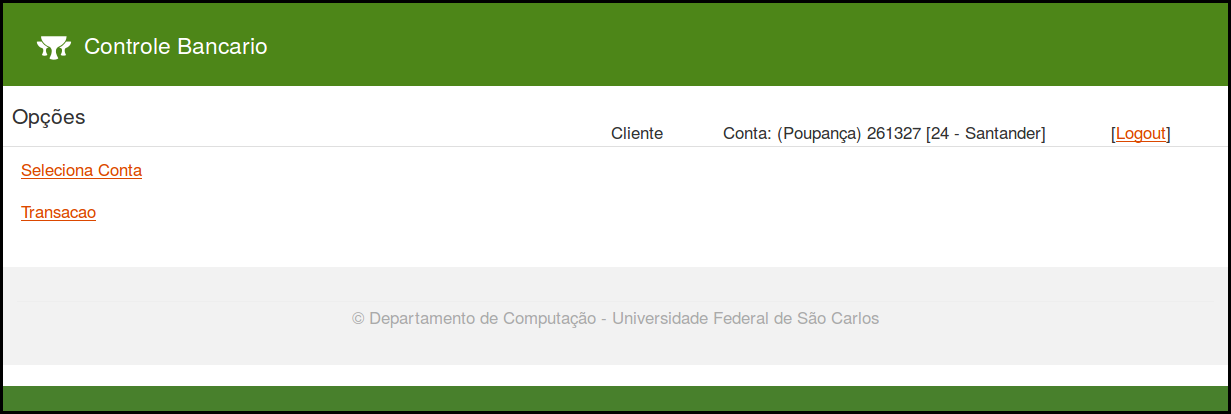
\includegraphics[width=14cm]{pageCliente}
\caption{Visão {\bf main/index.gsp}: {\bf ROLE\_CLIENTE}}
\label{figPageCliente}
\end{figure}

Conforme pode-se  observar o  usuário {\it logado}  tem duas  opções disponíveis
(dois controladores da aplicação {\bf ControleBancario}):

\vspace{0.3cm}

\begin{itemize}

\item {\bf SelecionaConta} caso deseje escolher que conta (corrente ou poupança)
  ele deseja acessar;

\vspace{0.3cm}

\item  {\bf  Transacao} caso  deseje  acessar/atualizar  a  lista de  transações
  realizadas    na    conta    que    está   sendo    acessada    no    momento.
  Figura~\ref{indexTransacaoFig}  apresenta a lista  de transações  associadas a
  uma conta do usuário {\it logado}.  

\end{itemize}

\begin{figure}[htbp]
\centering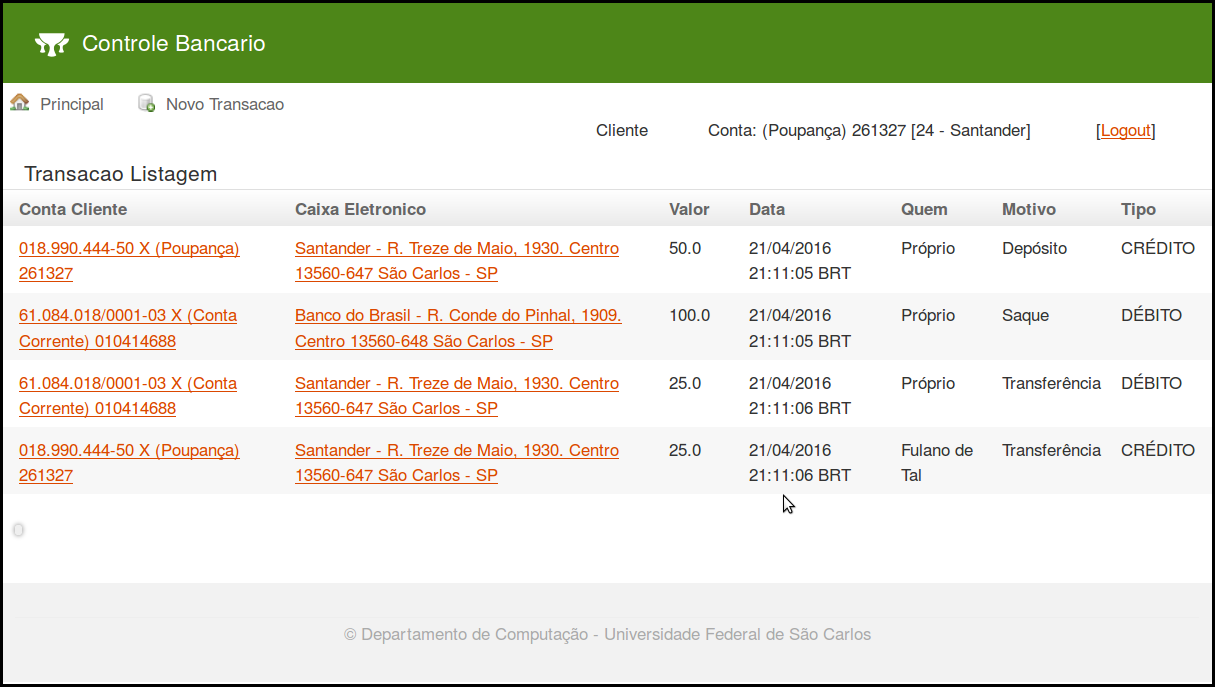
\includegraphics[width=14cm]{indexTransacao}
\caption{Lista de transações de uma conta do usuário {\it logado}}
\label{indexTransacaoFig}
\end{figure}

\section{Controle de acesso: Contas}

\vspace{0.5cm}

Conforme discutido no Capítulo~\ref{autenticacao}, o acesso às contas é restrito
aos usuários que desempenham o  papel {\bf ROLE\_GERENTE}.  Porém essa abordagem
não  é suficiente  pois um  gerente pode  acessar todas  as contas  (corrente ou
poupança) independentemente se essa conta pertence ou não a sua agência.

\vspace{0.2cm}

Na  versão  da  aplicação  {\bf  ControleBancario},  discutida  nesse  capítulo,
gerentes  apenas  terão acesso  às  contas pertencentes  à  agência  em que  ele
trabalha. 

\subsection{Controlador: ContaCorrenteController}

\vspace{0.5cm}

Código~\ref{codContaCorrenteController}    apresenta   a    reimplementação   do
controlador {\bf ContaCorrenteController} com o objetivo de refletir as mudanças
relacionadas a nova abordagem de controle de acesso discutida nesse capítulo.  

\vspace{0.2cm}

Relembrando  a  discussão  da  Seção~\ref{secTransacaoController}, a  ação  {\bf
  index()} é responsável por retornar a lista de instâncias da classe de domínio
{\bf  ContaCorrente}.  No caso  da implementação  apresentada nesse  capítulo, a
lista é composta apenas pelas contas  correntes que pertencem à agência em que o
usuário {\it logado} trabalha (variável de sessão {\bf agencia}). 

\vspace{0.2cm}

Por  fim,  relembrando  a  discussão da  Seção~\ref{secTransacaoController2},  é
possível que  gerentes {\it logados}  acessem de forma indevida  (maliciosa) uma
conta não  associada à agência  em que trabalha.  Nesse contexto, as  ações {\bf
  edit()}  e {\bf delete()}  foram alteradas  com o  objetivo de  prevenir essas
atualizações indevidas.

\vspace{0.5cm}

\begin{remark}
Análogo    ao     controlador    {\bf    ContaCorrenteController},     o    {\bf
  ContaPoupancaController}  também  necessita  ser  alterado  para  refletir  as
mudanças relacionadas  a nova  abordagem de controle  de acesso  discutida nesse
capítulo. Fica como exercício para o leitor realizar tal alteração. 
\end{remark}

\newpage

\begin{lstlisting}[caption=Controlador       {\bf      ContaCorrenteController},
    frame=trBL, float=htbp, label=codContaCorrenteController] 
class ContaCorrenteController {

    // Demais a^çõ^es/atributos/m^é^todos do controlador ContaCorrenteController

    def index(Integer max) {
        params.max = Math.min(max ?: 10, 100)        

        def results = ContaCorrente.findAllByAgencia(session.agencia, params)

        respond results, model:[contaCorrenteCount: ContaCorrente.count()]
    }

    def edit(ContaCorrente contaCorrente) {
        
        if (contaCorrente != null && contaCorrente.agencia.id != session.agencia.id) {
            flash.message = message(code: 'springSecurity.denied.message', args: [message(code: 
                                    'contaCorrente.label', default: 'ContaCorrente'), contaCorrente.id])
            redirect action: "index"
        }

        respond contaCorrente
    }

    @Transactional
    def delete(ContaCorrente contaCorrente) {
        
        if (contaCorrente.agencia.id != session.agencia.id) {
            flash.message = message(code: 'springSecurity.denied.message', args: [message(code: 
                                    'contaCorrente.label', default: 'ContaCorrente'), contaCorrente.id])
            redirect action: "index"
            return
        }

        if (contaCorrente == null) {
            notFound()
            transactionStatus.setRollbackOnly()
            return
        }

        contaCorrente.delete flush:true

        request.withFormat {
            form {
                flash.message = message(code: 'default.deleted.message', args: [message(code: 
                                        'contaCorrente.label', default: 'ContaCorrente'), contaCorrente.id])
                redirect action:"index", method:"GET"
            }
            '*'{ render status: NO_CONTENT }
        }
    }
}
\end{lstlisting}

\subsection{Template contaCorrente/\_fields.gsp}

\vspace{0.5cm}

Essa   seção  apresenta  o   {\it  template}   {\bf  contaCorrente/\_fields.gsp}
(Código~\ref{codContaCorrenteFields})  que  será   utilizado  pela  visões  {\bf
  create.gsp}  e {\bf  edit.gsp} e  que contém  a personalização  na  entrada do
atributo {\bf agencia} da classe de domínio {\bf ContaCorrente}.  

\vspace{0.2cm}

Conforme pode-se observar, a conta corrente criada/editada sempre será associada
à agência  (variável de  sessão {\bf  agencia}) em que  trabalha o  usuário {\it
  logado}.

\vspace{0.5cm}

\begin{lstlisting}[caption={\it     Template}     {\bf    contaCorrente/\_fields.gsp},
    frame=trBL, float=htbp, label=codContaCorrenteFields]
<div class="fieldcontain ${hasErrors(bean: contaCorrente, field: 'agencia', 'error')} required">
    <label for="agencia">
        <g:message code="contaCorrente.agencia.label" default="Agencia"/>
        <span class="required-indicator">*</span>
    </label>
    <g:select id="agencia" name="agencia.id" from="${session.agencia}" optionKey="id" required=""
              value="${contaCorrente?.agencia?.id}" class="many-to-one"/>
</div>
\end{lstlisting}

\newpage

Código~\ref{codContaCorrenteCreate}  mostra  a  reimplementação  da  visão  {\bf
  contaCorrente/create.gsp}. Por questão de brevidade, apenas serão apresentadas
as mudanças realizadas nessa visão.  Pode-se observar que  o {\it  template} {\bf
  \_fields.gsp} é renderizado (linha 17) no contexto do formulário HTML definido 
pela  {\it tag}  {\bf g:form}  (linhas 15--25).   Dessa forma,  o  atributo {\bf
  agencia} é  incluído no formulário  através da renderização do  {\it template}
{\bf \_fields.gsp}  enquanto os demais são  incluídos através da  {\it tag} {\bf
  f:all} (linha 19).  

\begin{lstlisting}[caption={\bf    contaCorrente/create.gsp},
    frame=trBL, float=htbp, label=codContaCorrenteCreate, numbers=left]
<div id="create-contaCorrente" class="content scaffold-create" role="main">
    <h1><g:message code="default.create.label" args="[entityName]"/></h1>
    <g:if test="${flash.message}">
        <div class="message" role="status">${flash.message}</div>
    </g:if>
    <g:hasErrors bean="${this.contaCorrente}">
        <ul class="errors" role="alert">
            <g:eachError bean="${this.contaCorrente}" var="error">
                <li <g:if test="${error in org.springframework.validation.FieldError}">
                                 data-field-id="${error.field}"</g:if>><g:message
                        error="${error}"/></li>
            </g:eachError>
        </ul>
    </g:hasErrors>
    <g:form action="save">
        <fieldset class="form">
            <g:render template="fields"/>

            <f:all bean="contaCorrente" except="agencia"/>
        </fieldset>
        <fieldset class="buttons">
            <g:submitButton name="create" class="save"
                            value="${message(code: 'default.button.create.label', default: 'Create')}"/>
        </fieldset>
    </g:form>
</div>
\end{lstlisting}

\begin{remark}
Análogo    à    visão    {\bf    contaCorrente/create.gsp},   a    visão    {\bf
  contaCorrente/edit.gsp}  também necessita  ser alterada  para utilizar  o {\it
  template} {\bf \_fields.gsp}.  

Análogo  ao {\it  template} {\bf  contaCorrente/\_fields.gsp}, o  {\it template}
{\bf   contaPoupanca/\_fields.gsp}   (e    consequentemente   as   visões   {\bf
  contaPoupanca/create.gsp} e  {\bf contaPoupanca/edit.gsp}) também  precisa ser
definido com  o intuito de personalizar  a entrada do atributo  {\bf agencia} da
classe  de  domínio {\bf  ContaPoupanca}.  Fica  como  exercício para  o  leitor
realizar tais alterações.  
\end{remark}

\subsection{Controlador: ContaClienteController}

\vspace{0.2cm}

Código~\ref{codContaClienteController2}    apresenta   a    reimplementação   do
controlador {\bf ContaClienteController} com o objetivo de refletir as mudanças
relacionadas a nova abordagem de controle de acesso discutida nesse capítulo.  

\vspace{0.1cm}

\hyphenation{ContaCliente}

A ação {\bf index()} é responsável  por retornar a lista de instâncias da classe
de   domínio  {\bf   ContaCliente}   que  materializa   o  relacionamento   {\em
  muitos-para-muitos}  entre   as  classes  de   domínio  {\bf  Conta}   e  {\bf
  Cliente}. No caso da implementação apresentada nessa seção, a lista é composta
apenas pelas instâncias que estão associadas a contas que pertencem à agência em
que o usuário {\it logado} trabalha (variável de sessão {\bf agencia}).  

\vspace{0.1cm}

A ação {\bf save()} valida os dados  e caso, tenha sucesso, grava a instância no
banco de  dados. No caso da  implementação apresentada nessa seção,  a ação {\bf
  save()}  também habilita  o cliente  (torna-se um  usuário da  aplicação) caso
esteja desabilitado. No contexto da aplicação {\bf ControleBancario}, um cliente
apenas  torna-se  um  usuário (pode  realizar  a  operação  de {\it  login})  da
aplicação  caso  tenha  uma  conta  associada. Além  disso,  conforme  discutido
anteriormente, é possível  que gerentes {\it logados} acessem  de forma indevida
(maliciosa) instâncias dessa  classe de domínio.  Nesse contexto,  as ações {\bf
  edit()}  e {\bf delete()}  foram alteradas  com o  objetivo de  prevenir essas
atualizações indevidas.  

\begin{lstlisting}[caption=Controlador {\bf ContaClienteController}, frame=trBL,
    float=htbp, label=codContaClienteController2] 
class ContaClienteController {

    // Demais a^çõ^es/atributos/m^é^todos do controlador ContaClienteController

    def index(Integer max) {
        params.max = Math.min(max ?: 10, 100)
		
        def results = ContaCliente.findAll("from ContaCliente as cc where cc.conta.agencia = :agencia",
            [agencia: session.agencia])
		
        respond results, model:[contaClienteCount: ContaCliente.count()]
    }

    @Transactional
    def save(ContaCliente contaCliente) {
        if (contaCliente == null) {
            transactionStatus.setRollbackOnly()
            notFound()
            return
        }

        if (contaCliente.hasErrors()) {
            transactionStatus.setRollbackOnly()
            respond contaCliente.errors, view:'create'
            return
        }

        contaCliente.save flush:true
        def cliente = contaCliente.cliente
        if (!cliente.enabled) {
            cliente.enabled = true
            cliente.save flush:true
        }

        request.withFormat {
            form multipartForm {
                flash.message = message(code: 'default.created.message', args: [message(code: 'contaCliente.label', 
                                        default: 'ContaCliente'), contaCliente.id])
                redirect contaCliente
            }
            '*' { respond contaCliente, [status: CREATED] }
        }
    }

    def edit(ContaCliente contaCliente) {
        if (contaCliente != null && contaCliente.conta.agencia.id != session.agencia.id) {
            flash.message = message(code: 'springSecurity.denied.message', args: [message(code:
                    'contaCliente.label', default: 'ContaCliente'), contaCliente.id])
            redirect action: "index"
        }
        respond contaCliente
    }

    @Transactional
    def delete(ContaCliente contaCliente) {
        if (contaCliente != null && contaCliente.conta.agencia.id != session.agencia.id) {
            flash.message = message(code: 'springSecurity.denied.message', args: [message(code:
                    'contaCliente.label', default: 'ContaCliente'), contaCliente.id])
            redirect action: "index"
        }

        if (contaCliente == null) {
            transactionStatus.setRollbackOnly()
            notFound()
            return
        }
        contaCliente.delete flush: true

        request.withFormat {
            form multipartForm {
                flash.message = message(code: 'default.deleted.message', args: [message(code: 'contaCliente.label', default: 'ContaCliente'), contaCliente.id])
                redirect action: "index", method: "GET"
            }
            '*' { render status: NO_CONTENT }
        }
    }

}
\end{lstlisting}

\newpage

\subsection{Template contaCliente/\_fields.gsp}

\vspace{0.5cm}

Essa   seção  apresenta   o  {\it   template}   {\bf  contaCliente/\_fields.gsp}
(Código~\ref{codContaClienteFields})  que   será  utilizado  pela   visões  {\bf
  create.gsp}  e {\bf  edit.gsp} e  que  contém personalizações  na entrada  dos
atributos {\bf cliente} e {\bf conta} da classe de domínio {\bf ContaCliente}.  

\begin{lstlisting}[caption={\it   Template}   {\bf   contaCliente/\_fields.gsp},
    frame=trBL, float=htbp, label=codContaClienteFields, numbers=left] 
<%@ page import="br.ufscar.dc.dsw.Conta" %>
<%@ page import="br.ufscar.dc.dsw.ContaCliente" %>

<div class="fieldcontain ${hasErrors(bean: contaClienteInstance, field: 'cliente', 'error')} required">
    <label for="cliente">
        <g:message code="contaCliente.cliente.label" default="Cliente"/>
        <span class="required-indicator">*</span>
    </label>
    <g:select id="cliente" name="cliente.id" from="${br.ufscar.dc.dsw.Cliente.list()}" optionKey="id"
              required="" value="${contaClienteInstance?.cliente?.id}"
              disabled="${contaClienteInstance?.cliente?.id != null}" class="many-to-one"/>
</div>

<div class="fieldcontain ${hasErrors(bean: contaClienteInstance, field: 'conta', 'error')} required">
    <label for="conta">
        <g:message code="contaCliente.conta.label" default="Conta"/>
        <span class="required-indicator">*</span>
    </label>
    <g:set var="contas"
           value="${Conta.findAll("from Conta as conta where conta.agencia = ?", [session.agencia])}"/>
    <g:select id="conta" name="conta.id" from="${contas}" optionKey="id" required=""
              value="${contaClienteInstance?.conta?.id}"
              disabled="${contaClienteInstance?.conta?.id != null}" class="many-to-one"/>
</div>
\end{lstlisting}

Conforme pode-se  observar, os campos de  seleção dos atributos  {\bf cliente} e
{\bf conta} são desabilitados nas operações de edição (linhas 11 e 23) -- quando
o  relacionamento {\em  muitos-para-muitos}  entre as  classes  de domínio  {\bf
  Conta} e  {\bf Cliente}  já foi  estabelecido.  Ou seja,  na edição  apenas os
demais atributos podem  ser atualizados. Além disso, o  segundo campo de seleção
(linha 21) apenas possibilita que o usuário {\it logado} apenas possa selecionar
contas (corrente ou  poupança) pertencentes à agência em  que trabalha (variável
de sessão {\bf agencia}).  

\vspace{0.2cm}

Código~\ref{codContaClienteCreate}  mostra  a   reimplementação  da  visão  {\bf
  contaCliente/create.gsp}. Por questão  de brevidade, apenas serão apresentadas
as mudanças realizadas nessa visão.   Pode-se observar que o {\it template} {\bf
  \_fields.gsp} é renderizado (linha 3)  no contexto do formulário HTML definido
pela {\it  tag} {\bf g:form}.   Dessa forma, os  atributos {\bf cliente}  e {\bf
  conta} são incluídos  no formulário através da renderização  do {\it template}
{\bf \_fields.gsp}  enquanto os demais são  incluídos através da  {\it tag} {\bf
  f:all} (linha 5).  

\begin{lstlisting}[caption={\bf    contaCliente/create.gsp},
    frame=trBL, float=htbp, label=codContaClienteCreate, numbers=left]
<g:form action="save">
    <fieldset class="form">
        <g:render template="fields"/>

        <f:all bean="contaCliente" except="cliente, conta"/>
    </fieldset>

    <fieldset class="buttons">
        <g:submitButton name="create" class="save"
                        value="${message(code: 'default.button.create.label', default: 'Create')}"/>
    </fieldset>
</g:form>
\end{lstlisting}

\begin{remark}
Análogo    à    visão    {\bf    contaCliente/create.gsp},    a    visão    {\bf
  contaCliente/edit.gsp}  também necessita  ser  alterada para  utilizar o  {\it
  template} {\bf \_fields.gsp}.  Fica como exercício para o  leitor realizar tal
alteração. 
\end{remark}

\subsection{Controlador: ContaController}

\vspace{0.5cm}

Código~\ref{codContaController2} apresenta a reimplementação do controlador {\bf
  ContaController} com  o objetivo de  refletir as mudanças relacionadas  a nova
abordagem de controle de acesso discutida nesse capítulo.  

\vspace{0.2cm}

Relembrando  a  discussão  da  Seção~\ref{secTransacaoController}, a  ação  {\bf
  index()} é responsável por retornar a lista de instâncias da classe de domínio
{\bf Conta}.   No caso  da implementação apresentada  nesse capítulo, a  lista é
composta  apenas pelas  contas que  pertencem à  agência em  que o  usuário {\it
  logado} trabalha (variável de sessão {\bf agencia}).

\begin{lstlisting}[caption=Controlador    {\bf   ContaController},   frame=trBL,
    float=htbp, label=codContaController2] 
class ContaController {

    // Demais a^çõ^es/atributos/m^é^todos do controlador ContaController
    
    def index(Integer max) {
        params.max = Math.min(max ?: 10, 100)
        
        def results = Conta.findAllByAgencia(session.agencia, params)
                
        respond results, model:[list: results, contaInstanceCount: Conta.count()]
    }
    
    @Secured(['ROLE_ADMIN', 'ROLE_CLIENTE', 'ROLE_GERENTE'])
    def show() {
        Conta conta = Conta.get(params.id)
        if (conta.instanceOf(ContaCorrente)) {
            forward controller: 'contaCorrente', action: "show"
        } else {
            forward controller: 'contaPoupanca', action: "show"
        }
    }
}

\end{lstlisting}

\subsection{Executando a aplicação}

\vspace{0.5cm}

Figura~\ref{figPageGerente} apresenta  a página principal  conforme acessada por
um usuário {\it logado} que desempenha o papel {\bf ROLE\_GERENTE}. 

\vspace{0.2cm}

\begin{figure}[htbp]
\centering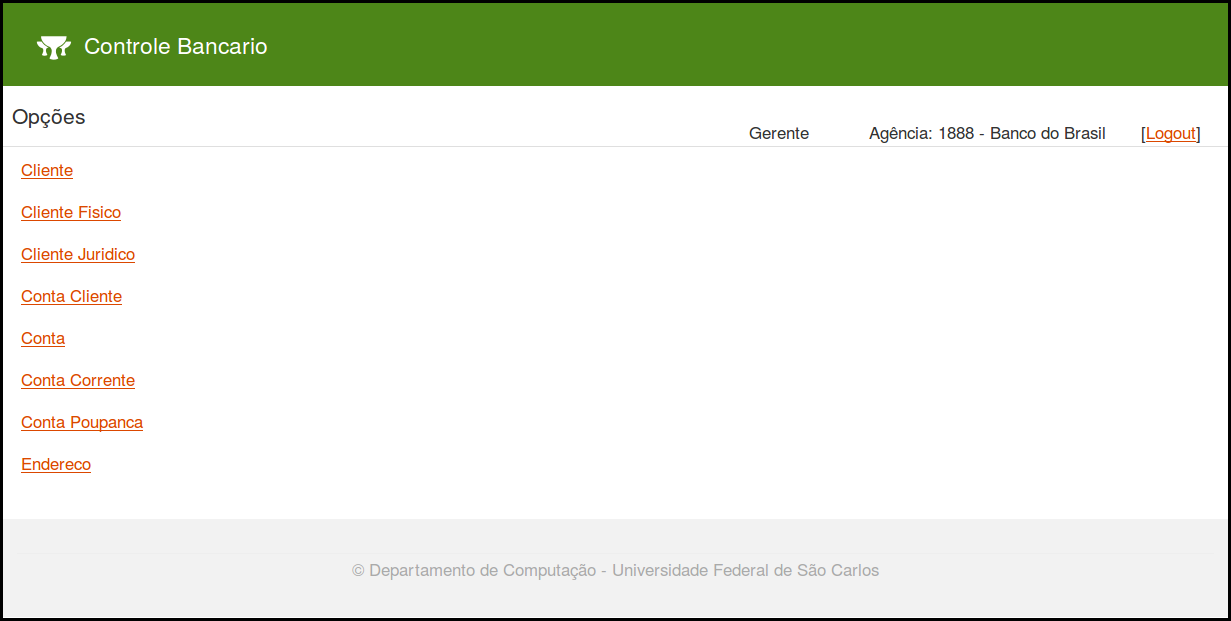
\includegraphics[width=14cm]{pageGerente}
\caption{Visão {\bf main/index.gsp}: {\bf ROLE\_GERENTE}}
\label{figPageGerente}
\end{figure}

Conforme pode-se  observar o  usuário {\it logado}  tem oito  opções disponíveis
(controladores da aplicação {\bf ControleBancario}): 

\vspace{0.4cm}

\begin{itemize}

\item  {\bf Cliente}, {\bf  ClienteFisico} e  {\bf ClienteJuridico}  caso deseje
  acessar/atualizar a lista  de clientes. Figura~\ref{indexClienteFig} apresenta
  a lista de clientes cadastrados na aplicação {\bf ControleBancario}.

\end{itemize}

\vspace{0.4cm}

\begin{figure}[htbp]
\centering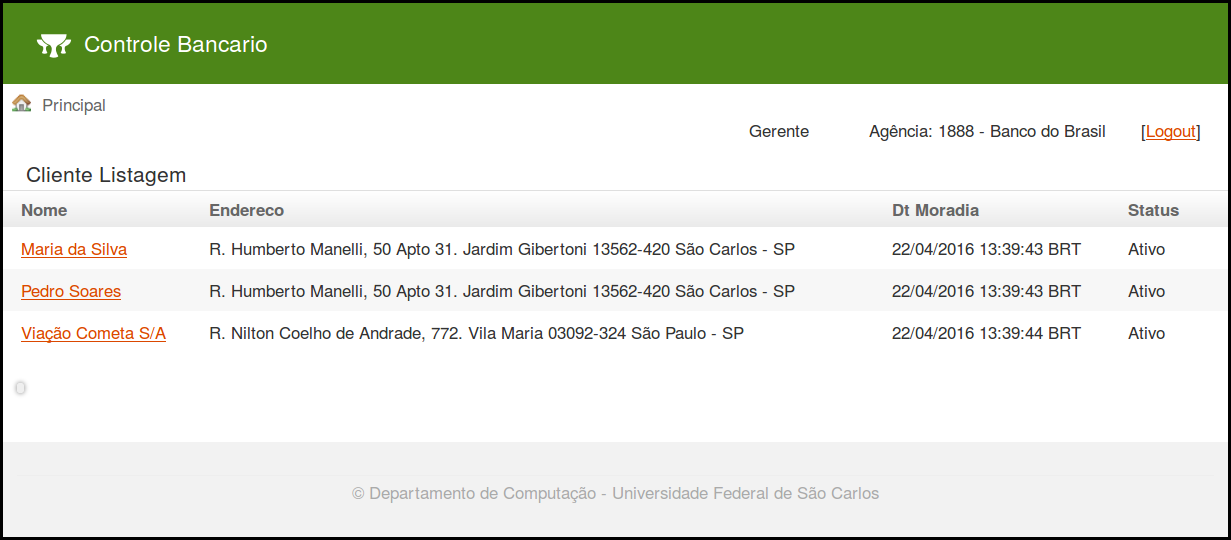
\includegraphics[width=14cm]{indexCliente}
\caption{Lista de clientes}
\label{indexClienteFig}
\end{figure}

\vspace{0.4cm}

\begin{itemize}

\item   {\bf   ContaCliente}   caso   deseje  acessar/atualizar   a   lista   de
  relacionamentos entre clientes e contas da agência do usuário {\it logado};

\vspace{0.4cm}

\item  {\bf  Conta},  {\bf  ContaCorrente}  e {\bf  ContaPoupança}  caso  deseje
  acessar/atualizar  a lista  de  contas  da agência  do  usuário {\it  logado}.
  Figura~\ref{indexContaFig} apresenta  a lista de contas da  agência do usuário
  {\it logado}.  

\end{itemize}

\vspace{0.4cm}

\begin{itemize}

\begin{figure}[htbp]
\centering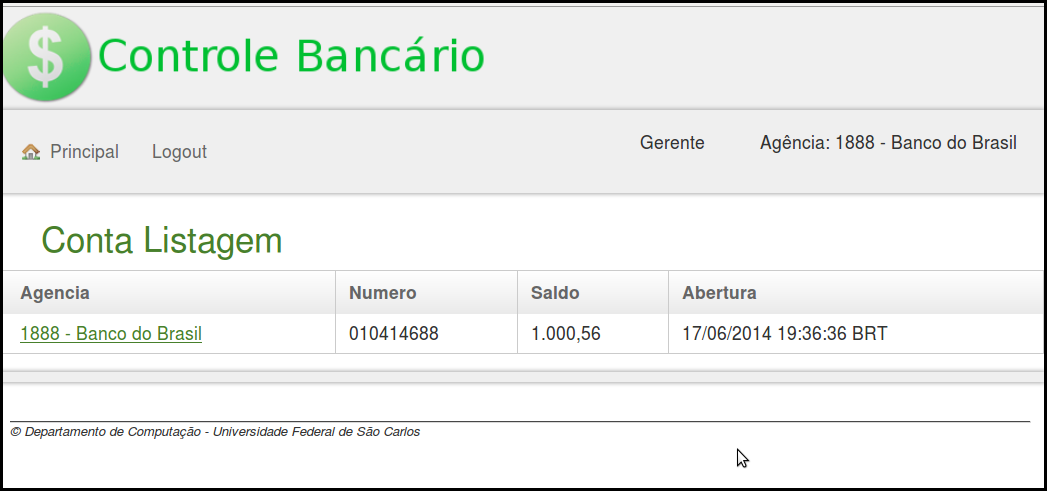
\includegraphics[width=14cm]{indexConta}
\caption{Lista de contas da agência do usuário {\it logado}}
\label{indexContaFig}
\end{figure}

\vspace{0.4cm}

\item  {\bf  Endereco}  caso  deseje  acessar/atualizar  a  lista  de  endereços
  cadastrados.
 
\end{itemize}

\newpage

\section{Preenchimento automático de endereços}\label{secAutoFill}

\vspace{0.5cm}

Essa seção  tem como objetivo  incorporar, na aplicação  {\bf ControleBancario},
algumas funcionalidades AJAX  relacionadas ao acesso a um  serviço {\it web}. Em
especial,   essa  seção   apresenta   a  implementação   da  funcionalidade   de
preenchimento automático dos atributos da classe de domínio {\bf Endereco}. 

\vspace{0.2cm}

Ou seja, dado o atributo CEP,  os demais atributos desse classe de domínio serão
preenchidos automaticamente.  Para prover  essa funcionalidade, será acessado um
serviço {\it web} que, dado um CEP como parâmetro, retorna as demais informações
de um endereço (logradouro, bairro, cidade, etc).  

\subsection{Template endereco/\_address.gsp}

\vspace{0.5cm}

O primeiro passo na  implementação da funcionalidade de preenchimento automático
de endereços  consiste em definir o {\it  template} {\bf endereco/\_address.gsp}
conforme  apresentado no  Código~\ref{codTemplateAddress}.  Esse {\it  template}
será utilizado pelas visões {\bf create.gsp}  e {\bf edit.gsp} e contém todos os
campos (exceto  o campo  CEP discutido a  seguir nessa seção)  responsáveis pela
entrada dos valores dos atributos da classe de domínio {\bf Endereco}.  

\begin{lstlisting}[caption={\it Template} {\bf endereco/\_address.gsp}, frame=trBL,
    float=htbp, label=codTemplateAddress] 
<%@ page import="br.ufscar.dc.dsw.Endereco" %>

<div class="fieldcontain ${hasErrors(bean: endereco, field: 'logradouro', 'error')}">
    <label for="logradouro">
        <g:message code="endereco.logradouro.label" default="Logradouro" />
    </label>
    <g:textField name="logradouro" maxlength="30" value="${endereco?.logradouro}"/>
</div>

<div class="fieldcontain ${hasErrors(bean: endereco, field: 'numero', 'error')}">
    <label for="numero">
        <g:message code="endereco.numero.label" default="Numero" />
    </label>
    <g:field name="numero" type="number" min="0" value="${endereco.numero}"/>
</div>

<div class="fieldcontain ${hasErrors(bean: endereco, field: 'complemento', 'error')} ">
    <label for="complemento">
        <g:message code="endereco.complemento.label" default="Complemento" />

    </label>
    <g:textField name="complemento" maxlength="20" value="${endereco?.complemento}"/>
</div>

<div class="fieldcontain ${hasErrors(bean: endereco, field: 'bairro', 'error')} ">
    <label for="bairro">
        <g:message code="endereco.bairro.label" default="Bairro" />
    </label>
    <g:textField name="bairro" maxlength="20" value="${endereco?.bairro}"/>
</div>

<div class="fieldcontain ${hasErrors(bean: endereco, field: 'cidade', 'error')} ">
    <label for="cidade">
        <g:message code="endereco.cidade.label" default="Cidade" />
    </label>
    <g:select id="cidade" name="cidade.id" from="${br.ufscar.dc.dsw.Cidade.list()}" optionKey="id" 
                          value="${endereco?.cidade?.id}" class="many-to-one"/>
</div>
\end{lstlisting}

Código~\ref{codEnderecoCreate}   mostra   a   reimplementação  da   visão   {\bf
  endereco/create.gsp}. Por  questão de brevidade, apenas  serão apresentadas as
mudanças realizadas  nessa visão.   Pode-se observar que  o {\it  template} {\bf
  \_address.gsp}  é  renderizado  (linha  15)  no contexto  do  formulário  HTML
definido pela {\it tag} {\bf g:form}. 

\newpage

No contexto  do formulário  foi definido  também, o campo  de texto  CEP (linhas
22-24)   de   tal  forma   que   o   tratamento   ao  evento   Javascript   {\it
  onblur}\footnote{O evento {\it onblur} ocorre  quando um objeto perde o foco.}
consiste em invocar, passando como parâmetro o conteúdo do campo de texto CEP, a
ação    {\bf   addressByCEP()}    do   controlador    {\bf   EnderecoController}
(Seção~\ref{secEnderecoController}).  

\begin{lstlisting}[caption={\bf endereco/create.gsp},
    frame=trBL, float=htbp, label=codEnderecoCreate, numbers=left]
<div id="create-endereco" class="content scaffold-create" role="main">
    <h1><g:message code="default.create.label" args="[entityName]" /></h1>
    <g:if test="${flash.message}">
       <div class="message" role="status">${flash.message}</div>
    </g:if>
    <g:hasErrors bean="${this.endereco}">
        <ul class="errors" role="alert">
            <g:eachError bean="${this.endereco}" var="error">
                <li <g:if test="${error in org.springframework.validation.FieldError}">
                                  data-field-id="${error.field}"</g:if>><g:message error="${error}"/></li>
            </g:eachError>
        </ul>
    </g:hasErrors>
    <g:form action="save">
       <fieldset class="form">

          <div class="fieldcontain ${hasErrors(bean: endereco, field: 'CEP', 'error')} required">
                <label for="CEP">
                    <g:message code="endereco.CEP.label" default="CEP" />
                    <span class="required-indicator">*</span>
                 </label>
                 <g:textField name="CEP" maxlength="9" required="" value="${endereco?.CEP}"
                           onblur="${remoteFunction(action: 'addressByCEP', update: [success: 'addressContainer'],
                                   params: '\'cep=\' + this.value', asynchronous: false)}"/>
           </div>

           <div id="addressContainer">
                <g:render template="address" bean="${endereco}"/>
           </div>

        </fieldset>
        <fieldset class="buttons">
             <g:submitButton name="create" class="save" 
                             value="${message(code: 'default.button.create.label', default: 'Create')}" />
        </fieldset>
    </g:form>
</div>
\end{lstlisting}

O  {\it template} {\bf  endereco/\_address.gsp} será  atualizado em  resposta ao
retorno  da   invocação  da  ação  {\bf  addressByCEP()}   do  controlador  {\bf
  EnderecoController}.   Ou  seja,  as  informações retornadas  pela  ação  {\bf
  addressByCEP()}  serão utilizados  para o  prenchimento automático  dos demais
atributos da classe de domínio {\bf Endereco}.  

\vspace{0.2cm}

É importante salientar que  o {\it template} {\bf endereco/\_address.gsp} apenas
será atualizado pois encontra-se no escopo  de uma {\it tag} {\bf div} cujo {\bf
  id} ({\it addressContainer}) é igual ao valor do atributo {\bf update/success}
de {\bf remoteFunction} (Código~\ref{codEnderecoCreate}, linhas 23 e 27). 

\vspace{0.2cm}

\begin{remark}
Análogo  à  visão {\bf  endereco/create.gsp},  a  visão {\bf  endereco/edit.gsp}
também   necessita  ser   alterada   para  utilizar   o   {\it  template}   {\bf
  \_address.gsp}.  Fica como exercício para o leitor realizar tal alteração. 
\end{remark}

\newpage

\subsection{Controlador: EnderecoController}
\index{Serviços {\it web} REST!Cliente}
\label{secEnderecoController}

\vspace{0.5cm}

O segundo  passo na implementação da funcionalidade  de preenchimento automático
de endereços consiste  em implementar a ação {\bf  addressByCEP()} que, conforme
discutido    anteriormente,    é    invocado    pelo   {\it    template}    {\bf
  endereco/\_address.gsp} (Código~\ref{codEnderecoController}). 

\vspace{0.2cm}

\hyphenation{addressByCEP}

Essa  ação   utiliza  as  funcionalidades   providas  pelo  {\it   plugin}  {\bf
  grails-datastore-rest-client} que  possibilita o  acesso a serviços  {\it web}
REST.  Ou seja, conforme pode-se observar, a ação {\bf addressByCEP~()} invoca um
serviço  {\it web}  REST que,  dado  um CEP  como parâmetro,  retorna as  demais
informações de um endereço (logradouro, bairro, cidade, etc).  

\vspace{0.2cm}

O  serviço {\it  web} REST  retorna  o endereço  em formato  JSON\footnote{JSON,
  acrônimo  para  {\it JavaScript  Object  Notation},  é  um formato  leve  para
  intercâmbio de dados computacionais.} com as seguintes informações: 

\vspace{0.3cm}

\begin{itemize}

\item {\bf uf} que armazena a sigla da unidade federativa/estado;

\vspace{0.3cm}

\item {\bf cidade} que armazena o nome da cidade;

\vspace{0.3cm}

\item {\bf bairro} que armazena o nome do bairro;

\vspace{0.3cm}

\item {\bf  tipo\_logradouro} que armazena  o tipo do logradouro  (rua, avenida,
  etc); e

\vspace{0.3cm}

\item {\bf logradouro} que armazena o nome do logradouro.

\end{itemize}

\begin{lstlisting}[caption=Controlador  {\bf EnderecoController}, frame  = trBL,
    float=htbp, label=codEnderecoController] 
class EnderecoController {

    // Demais a^çõ^es/atributos/m^é^todos do controlador EnderecoController

    def addressByCEP() {

        String restUrl="http://cep.republicavirtual.com.br/web_cep.php?cep="+params.cep+"&formato=json"

        RestBuilder rBuilder = new RestBuilder()
        RestResponse rResponse = rBuilder.get(restUrl)

        def html = rResponse?.json
        params.estado = Estado.findBySigla(html.uf)
        params.cidade = Cidade.findByNomeAndEstado(html.cidade, params.estado)
        params.bairro = html.bairro
        params.logradouro = html.tipo_logradouro + " " + html.logradouro

        render template: 'address', model: [endereco: new Endereco(params)]
    }
}
\end{lstlisting}

\vspace{0.3cm}

Tomando como base as informações retornadas  pelo serviço {\it web} REST, a ação
{\bf addressByCEP()}  cria uma instância da  classe de domínio  {\bf Endereco} e
retorna  essa   instância  para  ser   renderizada  pelo  {\it   template}  {\bf
  endereco/\_address.gsp}. 

\vspace{0.2cm}

Figura~\ref{figEnderecoCEP} apresenta a página de cadastro de um endereço (visão
{\bf endereco/create.gsp}) em que os  atributos {\bf logradouro}, {\bf bairro} e
{\bf cidade} foram preenchidos automaticamente pelas informações retornadas pela
ação {\bf addressByCEP()}.  

\vspace{0.3cm}

\begin{figure}[htbp]
\centering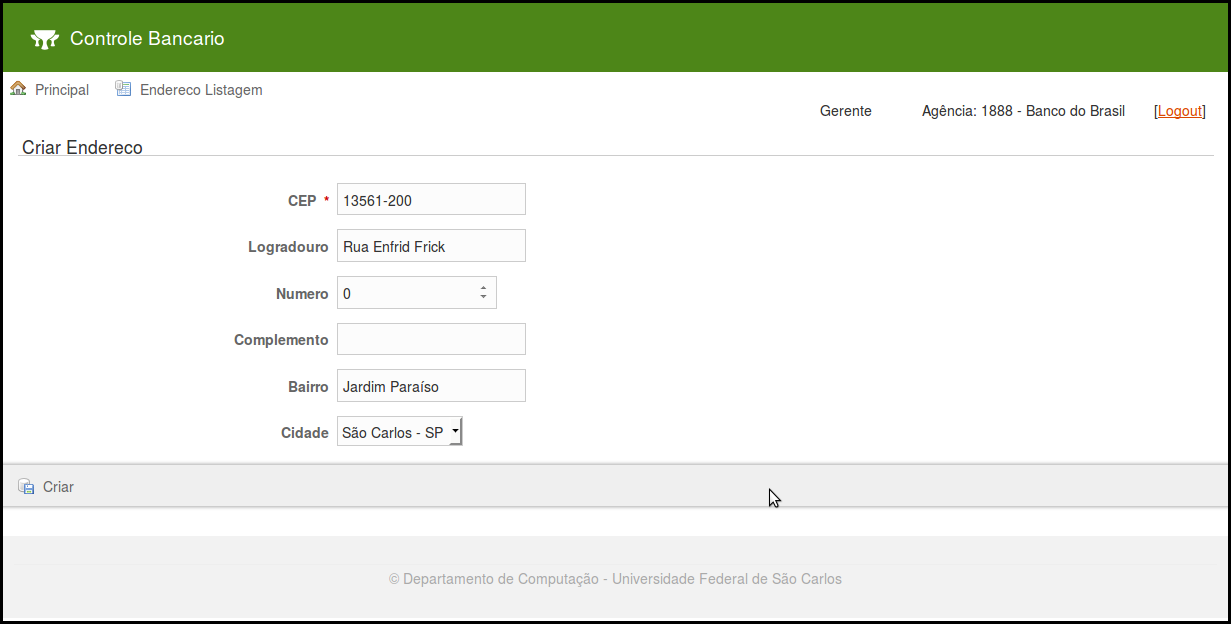
\includegraphics[width=14.5cm]{enderecoCEP}
\caption{Visão {\bf endereco/create.gsp}: Preenchimento automático de atributos}
\label{figEnderecoCEP}
\end{figure}

\newpage

\section{Considerações finais}

\vspace{0.3cm}

Esse capítulo  apresentou a terceira  versão da implementação da  aplicação {\bf
  ControleBancario}.         O        código-fonte        dessa        aplicação
({\footnotesize\texttt{ControleBancarioV3}})   encontra-se   disponível  em   um
repositório {\it GitHub}\footnote{URL: {\url{https://github.com/delanobeder/FG}}}.  

\vspace{0.2cm}

Dando  continuidade, o  próximo  capítulo  apresenta o  {\it  overview} de  mais
algumas  funcionalidades  presentes  em  Grails  que  não  foram  abordadas  nos
capítulos anteriores.  

